\section{\src{comp_caldyn_vert}}

\subsection{Description}

Kernel \src{comp_caldyn_vert} is taken from the original subroutine
\src{compute_caldyn_vert} in \DYNAMICO.
%
This subroutine is originally defined in module \src{caldyn_gcm_mod}.
%
This module defines subroutine \src{caldyn}, which is the main
subroutines for dynamics part of the model, and several sub-subroutines
for various terms in the governing equation, such as potential
vorticity, geopotential, etc.
%
This subroutine calculates vertical mass flux and vertical transport.



\subsection{Discretization and code}


\autoref{l:definition_comp_caldyn_vert} shows the definition part of this subroutine,
and \autoref{f:pad_comp_caldyn_vert} shows the PAD of this.


\begin{LstF90}[%
caption={Definition part of \src{compute_caldyn_vert}},%
label={l:definition_comp_caldyn_vert}%
]
SUBROUTINE compute_caldyn_vert(u,theta,rhodz,convm, wflux,wwuu, dps,dtheta_rhodz,du)
  USE icosa
  USE disvert_mod
  USE exner_mod
  USE trace
  USE omp_para
  IMPLICIT NONE
    REAL(rstd),INTENT(IN)  :: u(iim*3*jjm,llm)
    REAL(rstd),INTENT(IN)  :: theta(iim*jjm,llm)
    REAL(rstd),INTENT(IN)  :: rhodz(iim*jjm,llm)
    REAL(rstd),INTENT(INOUT)  :: convm(iim*jjm,llm)  ! mass flux convergence

    REAL(rstd),INTENT(INOUT) :: wflux(iim*jjm,llm+1) ! vertical mass flux (kg/m2/s)
    REAL(rstd),INTENT(INOUT) :: wwuu(iim*3*jjm,llm+1)
    REAL(rstd),INTENT(INOUT) :: du(iim*3*jjm,llm)
    REAL(rstd),INTENT(INOUT) :: dtheta_rhodz(iim*jjm,llm)
    REAL(rstd),INTENT(INOUT) :: dps(iim*jjm)

! temporary variable
    INTEGER :: i,j,ij,l
    REAL(rstd) :: p_ik, exner_ik
    INTEGER,SAVE ::ij_omp_begin, ij_omp_end
!$OMP THREADPRIVATE(ij_omp_begin, ij_omp_end)
    LOGICAL,SAVE :: first=.TRUE.
!$OMP THREADPRIVATE(first)
\end{LstF90}
%
Where \src{u}, \src{theta}, \src{rhodz} are wind velocity on the edge,
potential temperature, and mass, respectively.
\src{convm}, \src{wflux}, \src{wwuu} are mass flux convergence, vertical mass flux,
and \src{wflux*u} on the edge, respectively.
%
Last three variables are time derivatives.
\src{du}, \src{dtheta_rhodz}, \src{dps} are for wind velocity on the edge,
mass-weighted potential temperature, and surface pressure, respectively.
%
All of these except \src{dps} are two dimensional.
%
First dimension is for horizontal index, and the size depends on the
point where the variable is defined, since \DYNAMICO adopts C-grid.
%
Second dimension is for vertical index, and the size is \src{llm},
except \src{llm+1} for \src{wflux} and \src{wwuu}, these are defined on
the half level in vertical, while others are defined on the full level.

\begin{figure}[tbp]
 \centering
 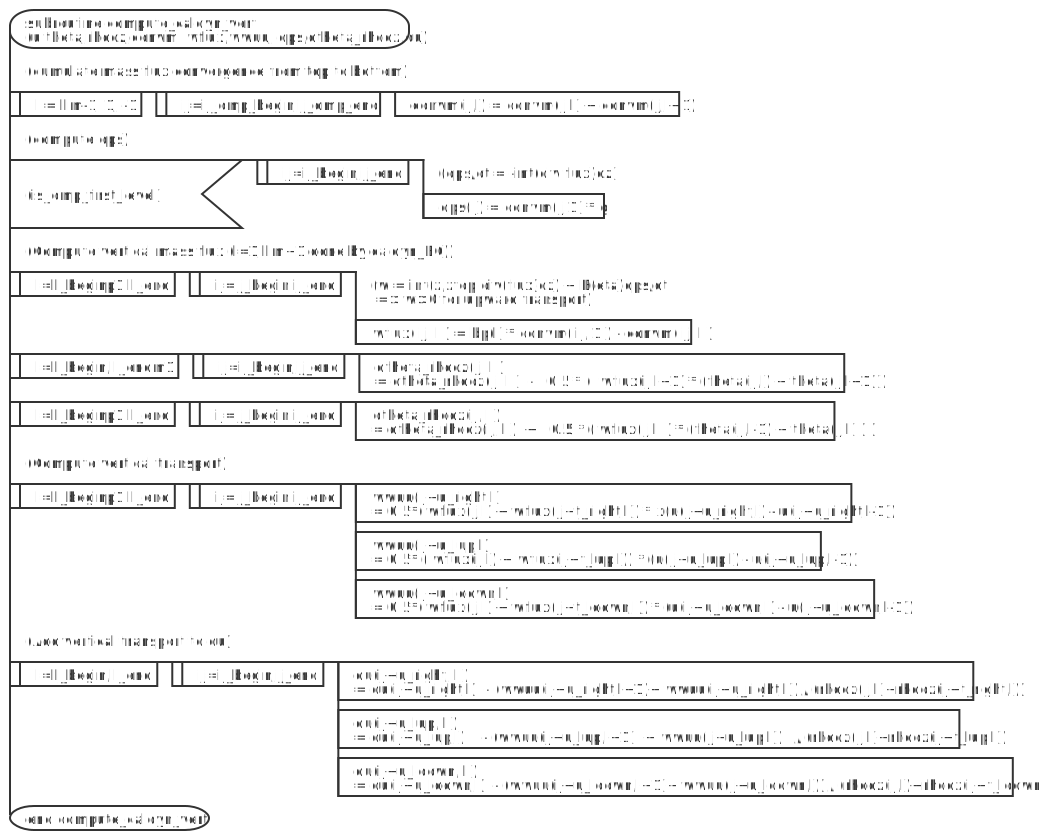
\includegraphics[scale=.5]{figs/caldyn_vert.pdf}
 \caption{PAD of \src{compute_caldyn_vert}}
 \label{f:pad_comp_caldyn_vert}
\end{figure}

Main part of this subroutine is consist of several $l$- and $ij$- double loop.
%
The first double loop is to accumulate mass flux convergence from top to bottom,
then convert \src{convm} at the lowest level to \src{dps}.
%
The second double loop is to compute vertical mass flux \src{wflux}.
%
Note that the range of $l$-loop, because \src{wflux} is defined on half
vertical level and at the top and the bottom are already set by
subroutine \src{caldyn_BC} as a boundary condition.
%
Next two double loop is to calculate convergence of potential
temperature \src{dtheta_rhodz}.
%
Again note that the range of two $l$-loop, since \src{dtheta_rhodz} is
defined on full vertical level and needs to sum up both upper and lower
face of the level.
%
Next two double loop is to compute vertical transport \src{wwuu}, and to
add it to \src{du}.
%
Note the horizontal index here.
%
\src{wwuu} and \src{du} are defined on the edge
of control volume, there are three statement in each double loop.

\clearpage



\subsection{Inputdata and result}

Input data file is prepared and you can download from official server using
\file{data/download.sh} script.
%
This data file is created by original \DYNAMICO\footnotemark with
Held-Suarez case parameter set included in the original source archive.
%
\footnotetext{with slight modification by AICS.}
%
Max/min/sum of input/output data of the kernel subroutine are output as
a log.
%
Below is an example of \src{$IAB_SYS=Ubuntu-gnu-ompi} case.

\begin{LstLog}
 [KERNEL] comp_caldyn_vert
 *** Start  initialize
                iim, jjm, llm:    23    25    19
             ij_begin, ij_end:    48   528
     ij_begin_ext, ij_end_ext:    24   552
             ll_begin, ll_end:     1    19
         ll_beginp1, ll_endm1:     2    18
        t_right, t_rup, t_lup:     1    23    22
     t_left, t_ldown, t_rdown:    -1   -23   -22
        u_right, u_rup, u_lup:     0  1173   575
     u_left, u_ldown, u_rdown:    -1  1150   553
           z_rup, z_up, z_lup:   598     0   597
     z_ldown, z_down, z_rdown:   -23   575   -22
                       dbg: g:     9.80000000
 +check[bp              ] max=  1.0000000000000000E+00,min=  0.0000000000000000E+00,sum=  6.9254510678414132E+00
 *** Finish initialize
 *** Start kernel
 ### check point iteration:        1000
 ### Input ###
 +check[u               ] max=  4.1278968179782127E-01,min= -4.1278968179782127E-01,sum=  1.6791131703073393E+01
 +check[theta           ] max=  8.0139914420291746E+02,min=  0.0000000000000000E+00,sum=  3.8582633571973117E+06
 +check[rhodz           ] max=  1.2306877011993038E+03,min=  0.0000000000000000E+00,sum=  5.3979591836733194E+06
 +check[convm_prev      ] max=  1.0361970643226587E-03,min= -1.0359249303947807E-04,sum= -1.5233533963107249E-01
 +check[wflux_prev      ] max=  0.0000000000000000E+00,min=  0.0000000000000000E+00,sum=  0.0000000000000000E+00
 +check[wwuu_prev       ] max=  0.0000000000000000E+00,min=  0.0000000000000000E+00,sum=  0.0000000000000000E+00
 +check[du_prev         ] max=  3.4404317002518906E-03,min= -3.0804630348046005E-03,sum=  5.5048589972605033E-01
 +check[dtheta_rhodz_pre] max=  3.2251351666935379E-01,min= -3.3676276308628725E-02,sum= -5.3720539414185993E+01
 +check[dps_prev        ] max=  0.0000000000000000E+00,min=  0.0000000000000000E+00,sum=  0.0000000000000000E+00
 ### Output ###
 +check[convm           ] max=  6.9593389571287302E-03,min= -7.9269107622801825E-04,sum= -1.5227927267389074E+00
 +check[wflux           ] max=  4.1171035230973149E-04,min= -3.6145630748324665E-03,sum=  5.8901163077820706E-01
 +check[wwuu            ] max=  1.7149300599654128E-04,min= -1.8768192515764522E-04,sum= -5.0377733672629036E-04
 +check[du              ] max=  3.4404317002518906E-03,min= -3.0804630348046005E-03,sum=  5.5048632410110032E-01
 +check[dtheta_rhodz    ] max=  3.5427038431326496E-01,min= -4.2032604085394595E-02,sum= -5.3720539414186263E+01
 +check[dps             ] max=  6.8201521779861565E-02,min= -7.7683725470345790E-03,sum= -1.3213658793877174E+00
 ### final iteration:        1000
 ### Validation : grid-by-grid diff ###
 +check[convm           ] max=  0.0000000000000000E+00,min=  0.0000000000000000E+00,sum=  0.0000000000000000E+00
 +check[wflux           ] max=  0.0000000000000000E+00,min=  0.0000000000000000E+00,sum=  0.0000000000000000E+00
 +check[wwuu            ] max=  0.0000000000000000E+00,min=  0.0000000000000000E+00,sum=  0.0000000000000000E+00
 +check[du              ] max=  0.0000000000000000E+00,min=  0.0000000000000000E+00,sum=  0.0000000000000000E+00
 +check[dtheta_rhodz    ] max=  0.0000000000000000E+00,min=  0.0000000000000000E+00,sum=  0.0000000000000000E+00
 +check[dps             ] max=  0.0000000000000000E+00,min=  0.0000000000000000E+00,sum=  0.0000000000000000E+00
 *** Finish kernel
\end{LstLog}

Check the lines below \src{``Validation : grid-by-grid diff''} line,
that shows difference between calculated output array and
pre-calculated reference array.
These should be zero or enough small to be acceptable.
%
There are sample output log files in \file{reference/}
in each kernel program directory, for reference purpose.

\subsection{Sample of performance result}

Here's an example of the performance result part of the log output.
Below is an example executed with the machine environment described in \autoref{s:measuring_env}.
%
Note that in this program kernel part is iterated 1000 times.

\begin{LstLog}
 *** Computational Time Report
 *** ID=001 : MAIN_comp_caldyn_vert            T=     0.156 N=   1000
\end{LstLog}

